\documentclass[12pt, letterpaper]{article}

\usepackage{graphicx}
\usepackage{amsmath}

\title{Experiment 5 Prelab}
\author{Jay Shen}
\date{April 2025}

\begin{document}

\begin{enumerate}

\maketitle

\item{
    See Figures \ref{fig:1.1} and \ref{fig:1.2}. 
    \begin{figure}
        \centering
        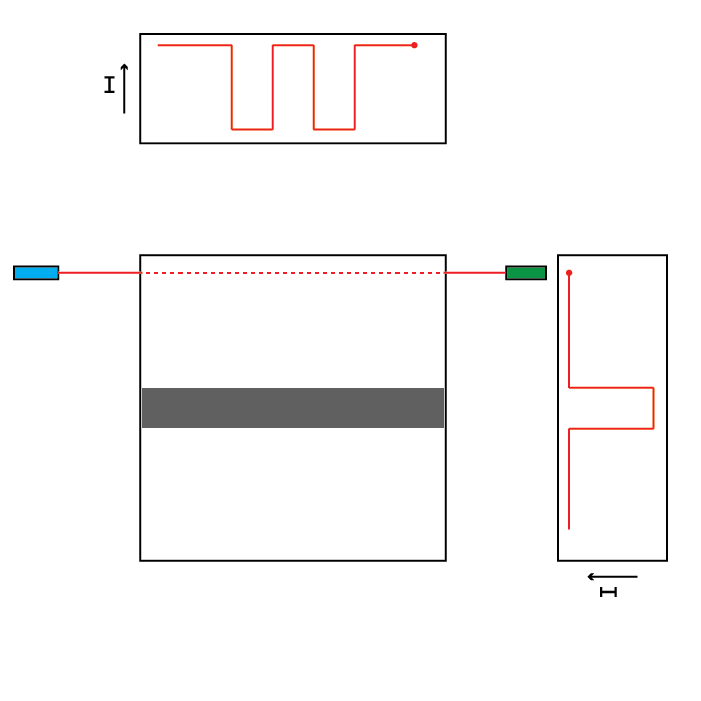
\includegraphics[width=0.4\linewidth]{experiment5/figures/prelab1-1.png}
        \caption{Part 1. The regions which may contain an object are highlighted in grey. }
        \label{fig:1.1}
    \end{figure}
    \begin{figure}
        \centering
        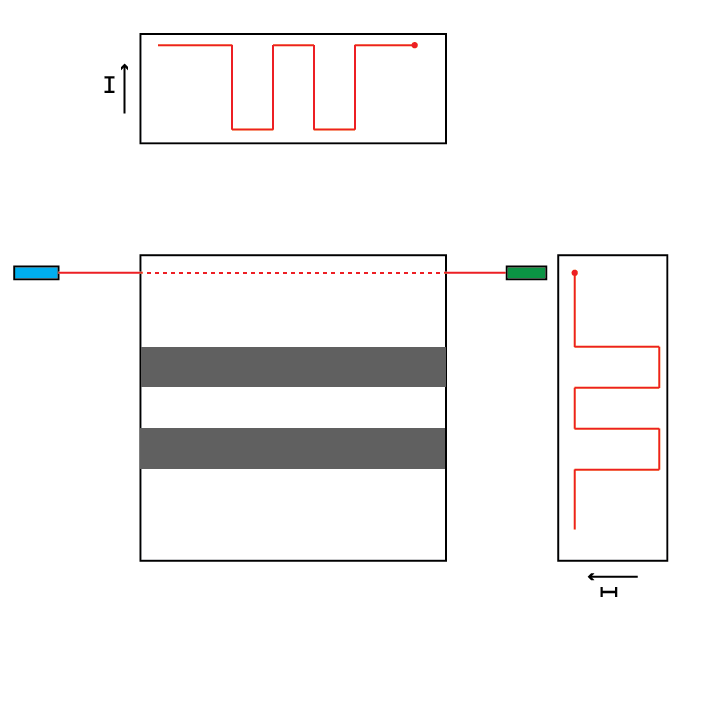
\includegraphics[width=0.4\linewidth]{experiment5/figures/prelab1-2.png}
        \caption{Part 2. The regions which may contain an object are highlighted in grey.}
        \label{fig:1.2}
    \end{figure}
}

\item{

    Source B can cause a balanced coincidence detection. Sources C, E can cause imbalanced coincidence detections. Sources D, A can cause a spurious coincidence detection. 

    Detector B can detect balanced coincidences. Detectors C, E can detect imbalanced coincidences. 

}
    
\end{enumerate}

\end{document}
